\begin{figure}[t!]
\centering
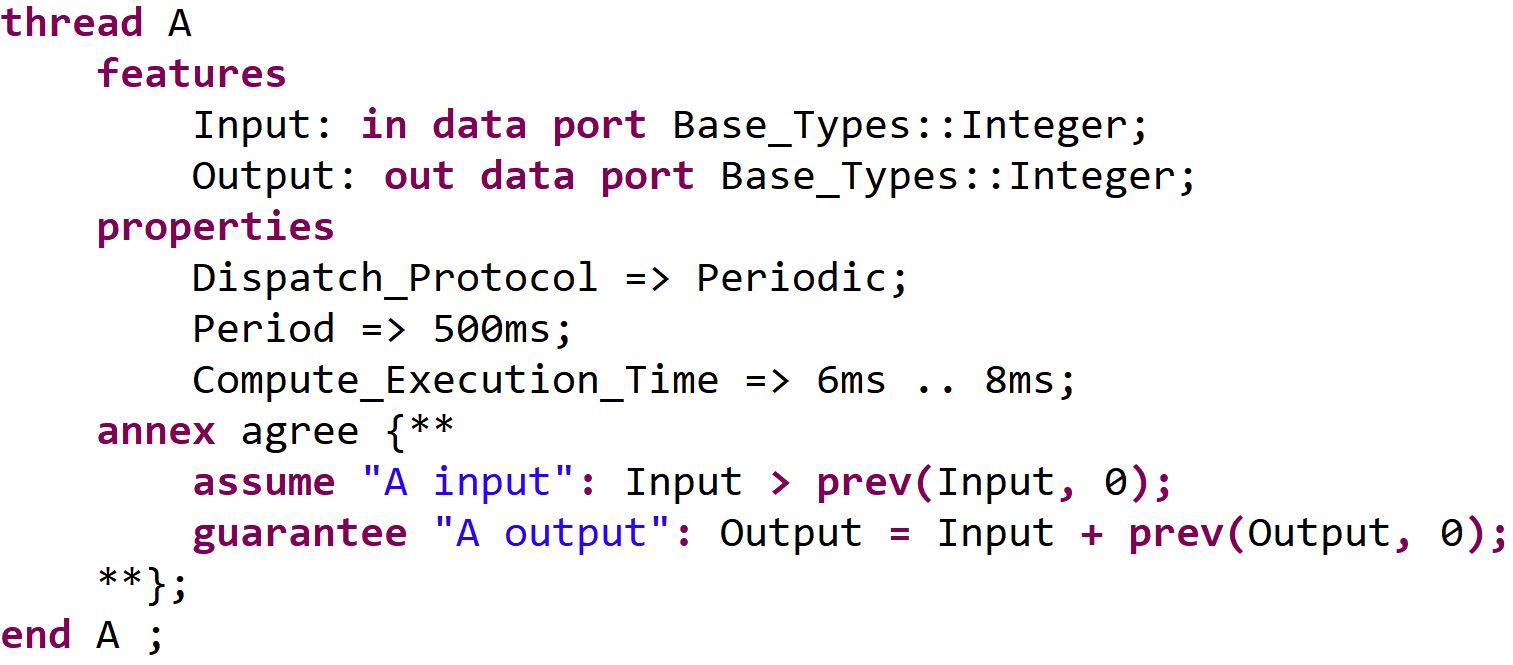
\includegraphics[width=80mm]{pre.jpg}
\caption{A Simple Integrator AADL Model in AGREE\label{integratorFig}}
\end{figure}

We now discuss in detail our semantic interpretation of AGREE contracts on scheduled components.
Consider the AADL model of an integrator, shown in Figure \ref{integratorFig}. We assume that an execution time slot is assigned to the thread.  
The first question that we face is when the contracts shall hold. In a synchronous model, contracts hold at every instant. However, with scheduled execution, it is reasonable to assume that the contract may not hold when the component is not activated. But once it is activated, shall a contract hold throughout the entire execution or just at certain instants? Second, how shall $Input$ (referred to in the contract) be interpreted? One interpretation is that it refers to the input value at the time when the contract is evaluated, which may vary during the execution. Another interpretation is that it refers to the input value when the component starts its execution. In other words, there is a notion of \emph{sample and hold}. This interpretation is consistent with the \emph{frozen} inputs described in the AADL V2 standard. Third, how shall the \emph{prev} operator be interpreted? In a synchronous model, it refers to the previous instant. However, with scheduled execution, it seems reasonable to interpret \emph{prev} as the previous activation (i.e. the value when the component was last activated). If the contracts hold throughout the activation, a more sensible interpretation is that at the first instant during activation, it refers to the previous activation. Then at each following instant, it refers to the last updated value in the current activation. This interpretation is adopted in the \emph{activation condition} in SCADE \cite{scade} and the \emph{clock} mechanism in SIGNAL \cite{signal}.

We believe that AGREE contracts are intended to model requirements \cite{AGREE2}, not implementations. Guarantees model the component requirements, and assumptions model the environmental constraints that are used to verify the component requirements. Following the AADL \emph{input-compute-output} model, assumptions are said to hold at the start of the execution (i.e. \emph{dispatch}) when the inputs are read. The guarantees shall be satisfied at the end of the execution (i.e. \emph{complete}) when the outputs are written. This interpretation has a few implications. 
First, since we adopt the AADL \textit{frozen inputs} concept, any reference to $Input$ refers to the input value that was read in at dispatch.
Second, a component's assigned time slot does not necessarily exactly match its execution time window. If the time slot is greater than its execution time, we interpret the start and end of the time slot as \textit{dispatch} and \textit{complete}, respectively. Otherwise, we claim that a \textit{preemption} has occurred.
Third, each contract is examined exactly once in each activation. Thus, we interpret the $prev$ operator as the previous activation. 
Fourth, the guarantees are not models of the \emph{transient} behavior during an execution. Instead, we interpret them as constraints on the \emph{steady-state} outputs at the end of activation.

%This is different from the real-time behavior models used to formalize AADL semantics, like real-time Maude \cite{maude}, timed automata \cite{behaviorannex}, and timed Petri net \cite{tpn}. They model the component timing behavior throughout the whole execution. 
We assume that the requirements do not contain real-time constraints. Modeling such constraints in AGREE is discussed in \cite{rtAGREE}.
However, this does not mean that AGREE contracts cannot model timer based requirements. In practice, a timer is usually implemented as a counter, whose limit (constant) is calculated based on the frequency of its execution. The counter is activated periodically and increments by only one during each activation, independent of the execution time. This is consistent with our interpretation.

Thus, for each component we introduce two distinctive events, \emph{dispatch} and \emph{complete}, to model the start and end of its activation, respectively. 
Similarly, for a system (consisting of components), the two events model the start and end of a scheduling cycle. 
The two events shall appear in pairs and alternate, with \emph{dispatch} appearing before \emph{complete}. We introduce the notion of \emph{well-ordered} in Section~\ref{async} to capture this pattern.

In SCADE and SIGNAL, when a component is not activated, its outputs retain their previous values. We extend this output freeze time window to \emph{complete} events, including activation. We understand that in practice the actual output values may change during activation. We choose this because we interpret the \emph{guarantees} as steady-state requirements of outputs at \emph{complete}. Output values between \textit{dispatch} and \textit{complete} are undefined. Thus, we model them using the last output values, so that the outputs are well-defined at every instant.

We inherit the same notion of composition used in the current AGREE framework. A connection between two components means their contracts refer to the same signal. 
This, combined with a schedule and the output freeze rule, essentially simulates communication based on \emph{shared variables}. When the producer is not activated, its outputs hold the last values. When the consumer is activated, it reads the last values from the producer. The communication may also be viewed as a FIFO queue, where the queue size is one. %The writer overwrites when overflow occurs. %The reader reads the previous value if the buffer is empty. 
This means the proposed model only supports limited AADL \textit{event} data port communication.
%This is consistent with the AADL data port sampling semantics. 

We only consider single-machine schedules. The scheduler ensures that at most one component is activated at a time. For a preemptive schedule, we require that a component can only be preempted by another component if they do not have connections. Thus, there is no ambiguity on the order of read and write or the variable value referenced in the contracts.

We assume that the system-level inputs do not change values throughout a scheduling cycle. In practice, this means that there may exist a queue that holds the system-level input messages, which are periodically sampled by the components, or the inputs may come from another system, which is inactive while the system under consideration is active.

The input freeze rule may imply that the assumptions could be examined at \emph{complete}, instead of \emph{dispatch}. Thus, we may not really need the \emph{dispatch} event. We keep it mainly for two reasons. First, the assumptions in general could depend on previous outputs. In our model, the outputs are updated at \emph{complete}. So the output values at \emph{dispatch} may be different from the values at the corresponding \emph{complete}. Therefore, it is important to distinguish between the two events to avoid ambiguity of the output values. Second, keeping the pair (\emph{dispatch}, \emph{complete}) may help users to better understand the AGREE counterexample trace, particularly with a preemptive schedule.

%{\bf Model of Real-Time Schedule.}
The original schedule is often specified in the form of a sequence of time slots assigned to the components. 
The schedule could come from an AADL real-time scheduling tool such as Cheddar \cite{cheddar}, or from a scheduler provided by an RTOS/Microkernel vendor, such as seL4 \cite{sel4}. 
To properly model the schedule in AGREE, the component execution time has to be considered. Consider the example shown in Figure \ref{RTschedule} with two scheduled components $A$ and $B$. We refer to the original schedule and its model in AGREE as the real-time schedule and AGREE schedule, respectively.
\begin{figure}[t!]
\centering
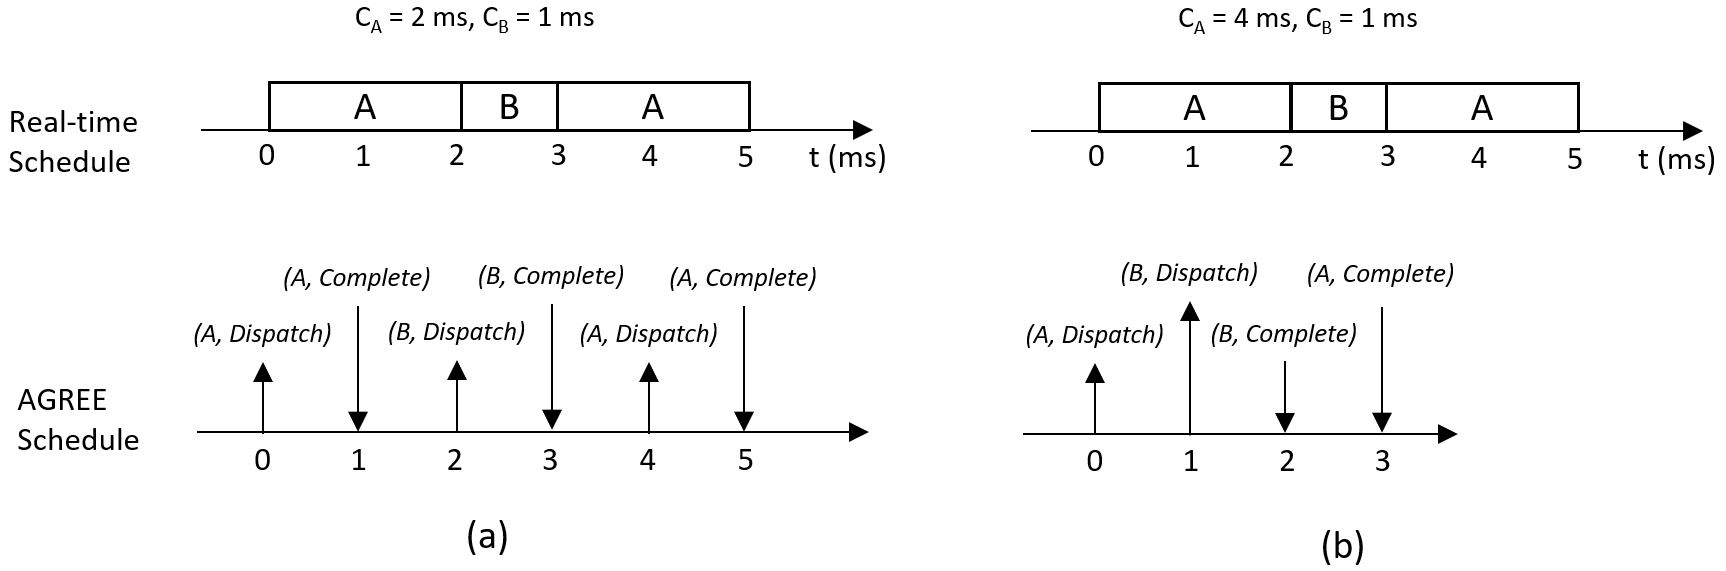
\includegraphics[width=\columnwidth]{RTschedule.jpg}
\caption{Models of Real-Time Schedule in AGREE\label{RTschedule}}
\end{figure}
Given the same real-time schedule, due to the different execution time $C_A$ of $A$, two different AGREE schedules are created. In Figure \ref{RTschedule}(a), since $C_A$ is equal to the time slots assigned to $A$, the end of the each time slot is modeled as \emph{complete}. In Figure \ref{RTschedule}(b), since the first time slot assigned to $A$ is less than its execution time, the end of the first time slot is interpreted as \emph{preemption}, instead of \emph{complete}.

%The AGREE reasoning framework uses past-time LTL [2], particularly LTL operator $G$ (globally), $H$ (historically), and $Z$ (previous). Given a component with an assume-guarantee pair ($A,P$) and an event pair (\emph{dispatch}, \emph{complete}), the meaning of the contract can be formally represented as a past-time LTL formula $G(H((dispatch \Rightarrow A)) \Rightarrow (complete \Rightarrow P))$. In synchronous AGREE, the two events \emph{collpase} into a single instant at each tick. Thus, we have $G(H(A) \Rightarrow P)$.


